% -*- latex -*-
%-----------------------------------------------------------------------
%;  Copyright (C) 2016
%;  Associated Universities, Inc. Washington DC, USA.
%;
%;  This program is free software; you can redistribute it and/or
%;  modify it under the terms of the GNU General Public License as
%;  published by the Free Software Foundation; either version 2 of
%;  the License, or (at your option) any later version.
%;
%;  This program is distributed in the hope that it will be useful,
%;  but WITHOUT ANY WARRANTY; without even the implied warranty of
%;  MERCHANTABILITY or FITNESS FOR A PARTICULAR PURPOSE.  See the
%;  GNU General Public License for more details.
%;
%;  You should have received a copy of the GNU General Public
%;  License along with this program; if not, write to the Free
%;  Software Foundation, Inc., 675 Massachusetts Ave, Cambridge,
%;  MA 02139, USA.
%;
%;  Correspondence concerning AIPS should be addressed as follows:
%;          Internet email: aipsmail@nrao.edu.
%;          Postal address: AIPS Project Office
%;                          National Radio Astronomy Observatory
%;                          520 Edgemont Road
%;                          Charlottesville, VA 22903-2475 USA
%-----------------------------------------------------------------------
%Body of final AIPSletter for 31 December 2016

\documentclass[twoside]{article}
\usepackage{graphics}

\newcommand{\AIPRELEASE}{December 31, 2016}
\newcommand{\AIPVOLUME}{Volume XXXVI}
\newcommand{\AIPNUMBER}{Number 2}
\newcommand{\RELEASENAME}{{\tt 31DEC16}}
\newcommand{\OLDNAME}{{\tt 31DEC15}}
\newcommand{\NEWNAME}{{\tt 31DEC17}}
\newcommand{\Tsys}{${\rm T}_{\rm sys}$}

%macros and title page format for the \AIPS\ letter.
\input LET98.MAC

\newcommand{\MYSpace}{-11pt}

\normalstyle

\section{General developments in \AIPS}

\subsection{Reduction of VLB, VLA and ALMA data in \AIPS}

\AIPS\ continues to be the main software system for the reduction of
VLBI data from the VLBA and other telescopes.  Since 2010, there have
been numerous improvements to \AIPS\ that enable full calibration of
data from the Karl G. Jansky VLA and most imaging operations as well.
The one exception is the wide-band (bandwidth synthesis) deconvolution
algorithm (``MSMFS'') being developed in \CASA\ by Urvashi Rao
Venkata, for which there is no comparable function in \AIPS\@.
Calibrated $uv$ data may be exported from \AIPS\ in ``UVFITS'' format
for use in that program.  ALMA data may also be reduced in \AIPS,
although the package is not fully qualified to calibrate data from
linearly-polarized feeds.  See Appendix E of the \AIPS\ Cookbook,
available via the \AIPS\ web site, for details.

\subsection{\Aipsletter\ publication}

We have discontinued paper copies of the \Aipsletter\ other than for
libraries and NRAO staff.  The \Aipsletter\ will be available in
PostScript and pdf forms as always from the web site listed above and
will be shipped with all distributions of \AIPS\@.  It will be
announced on the bananas and MNJ list servers and, usually, in the
NRAO e-News mailing.

\subsection{Current and future releases}

We have formal \AIPS\ releases on an annual basis.  We recommend a
full binary installation method for both the frozen and development
versions for MacIntosh OS/X (PPC and Intel chips), Solaris, and Linux
(32- and 64-bit) systems, but all architectures can do a full
installation from the source files.  If you develop \AIPS\ code
locally {\it or have system managers that forbid the use of\/} {\tt
  rsync} or {\tt cvs}, you will need to do a source-level
installation.  The current release is called \RELEASENAME\ and is now
``frozen.''  If you took a development copy of this version at some
earlier date, you should use the ``Midnight Job'' (MNJ) to bring it up
to date.  You need to run a MNJ only once in 2017 to convert your copy
of \RELEASENAME\ into the frozen version.  However, when patches to
\RELEASENAME\ are announced in 2017, you may apply them with the
MNJ\@.  This \Aipsletter\ is intended to advise you of corrections and
improvements in this release.

We have begun a new version, called \NEWNAME, which is now under
development by the \AIPS\ Group.  You may fetch and install a complete
copy of this version at any time.  Having fetched \NEWNAME, you may
update your installation whenever you want by running the MNJ\@.  This
uses {\tt cvs}, {\tt rsync}, and/or transaction files to copy all
changed text files and then to copy the binary files or to compile the
code selectively based on the code changes and compilations we have
done.  We expect users to take their source-only or binary version of
\NEWNAME\ \AIPS\ over the Internet (via \emph{anonymous} ftp).  Both
versions require you to copy the installation procedure {\tt
  install.pl} via {\tt ftp}; the source-only version also requires you
to ftp the 131-Mbyte {\tt   \NEWNAME.tar.gz} compressed tar file.
Binary installations use only {\tt rsync}, while locally compiled
versions also use {\tt cvs}.  Linux sites will almost certainly have
{\tt cvs} installed; other sites may have installed it along with
other GNU tools.  Secondary MNJs will still be possible using {\tt
  ssh} or {\tt rcp} or NFS as with previous releases.  We have found
that {\tt cvs} works very well, although it has one quirk. If a site
modifies a file locally, but in an \AIPS-standard directory, {\tt cvs}
will detect the modification and attempt to reconcile the local
version with the NRAO-supplied version.  This usually produces a file
that will not compile or run as intended.  Use a new name for the task
or put a copy of the task and its help file in a private disk area
instead.

\AIPS\ is now copyright \copyright\ 1995 through 2016 by Associated
Universities, Inc., NRAO's parent corporation, but may be made freely
available under the terms of the Free Software Foundation's General
Public License (GPL)\@.  This means that User Agreements are no longer
required, that \AIPS\ may be obtained via anonymous ftp without
contacting NRAO, and that the software may be redistributed (and/or
modified), under certain conditions.  The full text of the GPL can be
found in the \texttt{15JUL95} \Aipsletter\ and is included with every
distribution in file {\tt \$AIPS\_ROOT/{\it release-name}/COPYING}\@.


\subsection{Installing a new version}

If compiling locally, new releases must be installed from the tar ball
for that release.  {\tt 31DEC15} and later versions contain
improvements to the code which should make local compilation more
reliable.  If using the binary installation, a full new installation
must also be done with {\tt rsync}.  When installing a new \AIPS\
release in a system that already has a previous release, we recommend
that {\tt install.pl} be used and that the previous release be left in
place, at least until the new installation has been verified.  If you
do this, then you will not have to re-edit the disk, printer, and tape
lists and can simply skip all those pages in the {\tt install.pl}
menus.  The old {\tt \$HOME/.AIPSRC} file may be left in place, but it
will need to be edited.  The lines giving the {\tt DOWNLOADED} and
{\tt UNPACKED} parameters should be cleared and the {\tt CCOMOPT} line
should be changed to point to the current release rather than the
previous one.  If you have made a special version of {\tt
  do\_daily.{\it host}}, you should preserve it under a new name and
restore it after the install. If you have an odd set of \AIPS\
versions, the {\tt \$AIPS\_ROOT/AIPSPATH.*SH} files may need to be
edited after the install to set the desired versions.  The file {\tt
  \$SYSLOCAL/UPDCONFIG} also needs to be edited to correct your e-mail
address(es).

{\tt 31DEC09} contains a change in the format of antenna files.
Previous releases will not understand the antenna coordinates for
arrays that were traditionally left-handed (VLBI primarily).  The
format change occurs automatically when any {\tt 31DEC09} or later
antenna-file specific code reads the file, after which older releases
will have difficulties.  {\tt 31DEC15} contains a change in the
headers of $uv$ data sets which will not be understood by previous
versions.  Note that the only version which we patch for major errors
is \RELEASENAME; even \OLDNAME\ is no longer changed.

%\section{Preview of coming attractions}

%The \NEWNAME\ release already contains a few changes that we decided
%were a bit risky or not needed in \RELEASENAME\@.

%\vfill\eject
\section{Improvements of interest to users in \RELEASENAME}

In the first six months of \RELEASENAME\ the ```Midnight Job'' was
changed so that binary installations use only {\tt rsync}; {\tt cvs}
is no longer required.  A number of improvements to the MNJ were done
in the last six months in support of this change.  New tasks in this
period include {\tt UFLAG} to edit data interactively on a $uv$ grid,
{\tt BPEDT} to flag $uv$ data based on bandpass table problems found
interactively, {\tt FGTAB} to prepare fixed frequency flags for input
to {\tt UVFLG}, {\tt FGCNT} to compare the effects of two flag tables
on the amount of data remaining, and a suite of new tasks to handle
pulse-cal data for VLBI observations.  These are {\tt PCFLG} to edit a
{\tt PC} table with a frequency-time grey-scale display, {\tt PCEDT}
to edit a {\tt PC} table with a graphical display, {\tt PCPLT} to plot
{\tt PC} table spectra, {\tt PCASS} to compute bandpass correction
tables from {\tt PC} table data, and {\tt PCFIT} to write phase and
delay calibration information based on the {\tt PC} table phases.  Two
new verbs, {\tt TVCOMPS} and {\tt TVACOMPS} were added to plot slice
model components on the TV\@.  New tasks in in the first six months
include especially {\tt TVSPC} to review the contents of spectral
cubes interactively plus {\tt SLPRT} to print the contents of slice
files and {\tt UVGIT} to fit models to $uv$ data. The new verb {\tt
  DAYNUMBR} returns the day number in the year of the observation of
the cataloged file.

Normally, bugs which appear in an \AIPS\ {\tt TST} version and then
are fixed in that same version before its release get little or no
discussion in the \Aipsletter\@.  Since a rather large number of sites
now install the {\tt TST} version of \AIPS\ during its development,
this is somewhat of an oversight.  We urge you to run the ``Midnight
Job'' at least once after \RELEASENAME\ is frozen to bring it up to
date and to fix all bugs of this sort.  We urge active sites to use
the MNJ and, when something odd occurs, to examine {\tt CHANGE.DOC}
using the cgi tool available from the \AIPS\ documentation web page
({\tt http://www.aips.nrao.edu/aipsdoc.html}).  Please do not
hesitate to contact us via the NRAO help desk ({\tt
  https://help.nrao.edu}) or via e-mail {\tt daip@nrao.edu} with any
questions or suspicions that there are problems.

\subsection{UV data: Pulse-cal tables for VLBI}

The DiFX correlator is now capable of providing pulse-cal tones at
every MHz.  These complex data are written into text files archived in
full at the correlator site and may be written in the FITS-IDI output
files.  Since these data have very high signal-to-noise ratio, they
should be used wherever possible to assist with calibration.
Beginning in July 2016, AIPS was changed to support this capability.
In fact, AIPS can now handle up to 256 tones per spectral window,
which is way more than needed at present.  The first task changed for
these numerous pulse-cal tones was {\tt POSSM} which now offers an
option to plot pulse-cal spectra with its usual data averaging
options.  {\tt PCLOD} was also changed to read the new DiFX pulse-cal
text file format, writing a modern {\tt PC} table.

The pulse-cal spectra show both an amplitude shape resembling the
bandpass shape and "bad" channels, \ie\ channels with amplitudes and
phases differing from those expected from their neighbors.  Thus, new
tasks were written to edit the {\tt PC} tables.  {\tt PCFLG} is very
similar to {\tt SPFLG}, showing in gray-scale pulse-cal channel on the
X axis and time on the Y axis.  Unlike {\tt SPFLG}, which is used to
edit visibility data, {\tt PCFLG} writes out an edited version of the
input {\tt PC} table.  Numerous display types are available including
phase corrected for delay and phase fit to the input data (``residual
phase'').  The fits may be  re-done after some editing in case leaving
out the bad channels has a significant effect on the fits.  {\tt
  PCEDT} is a graphical editor to do the same operation.  The
graphical perspective is good, but if there is a large number of
times, editing with {\tt PCFLG} will be faster.  {\tt PCEDT} does
have the capability of computing and re-computing residual phases as
well.  Another new task, {\tt PCPLT}, resembles {\tt BPLOT} in that it
can plot pulse-cal spectra for all antennas, one time per page, or for
all times, one antenna per page.  This is another way to examine your
pulse-cal data to look for bad channels in amplitude, phase, or
residual phase with a variety of difference options as well.  Another
new task for pulse-cal data is {\tt PCFIT}, which does the fitting for
delay/phase and then writes out both a {\tt PC} table with residual
phases and an {\tt SN} table with either the fit delays and phases or
with the difference between the fits at time $t$ and the fits at the
first time in the {\tt PC} table.  It appears that the delays in the
{\tt PC} table are very large (100's of ns) and quite different
between antennas.  Thus, the fit delays are probably not suitable to
apply to the visibility data directly, but changes to the
pulse-cal delays are expected to reflect changes to the delay affecting
the visibility data.  Finally, another new task is called {\tt PCASS}
to compute bandpass-correction tables from the {\tt PC} table
amplitudes with or without the residual phases.

These new capabilities still need testing with real data, but they
offer significant opportunities for more accurate calibration of VLB
data.

\subsection{UV Data: Editing on a $uv$ grid and with bandpass tables}

When making images of newly-calibrated data, it is not uncommon to see
sine waves in the image particularly when Cleaning down toward the
image noise level.  Previously, to find the bad data, one had to use
tasks {\tt FFT} plus {\tt COMB} to make an image of the data on a $uv$
grid.  Then the $uv$ coordinates of the peaks in that image had to be
found and translated into locations in the visibility data set with
{\tt UVFND}\@.  Finally, {\tt UVFLG} had to be run multiple times.
This was tedious at best and not very reliable.

The whole process has now been replaced with the new task {\tt UFLAG}\@.
It grids selected visibility data onto a $uv$ grid and displays images
of the scalar average amplitude, the vector average amplitude, the
difference of these two, and the average phase, all of which may be
used to edit the data.  One may simply choose to flag a cell which
will flag all visibilities contributing to that cell.  But one may
also examine each of the visibilities contributing to a cell and flag
only those that you choose to delete.  There are even automated
methods to flag all visibilities outside desired ranges from cells
selected by various criteria.  All of these options are driven via a
TV menu plus question and answer sessions for the automated flagging.
The task is described fully in \AIPS\ Memo 121 (see below).

Another new task is {\tt BPEDT} with resembles {\tt EDITA} and
friends.  It uses a graphical display of bandpass table data with the
$X$ axis being frequency rather than time.  The amplitude or phase is
displayed in an edit window for the particular antenna and time, with
comparison windows of the other parameter for the particular antenna
and the same parameter for chosen comparison antennas.  Bad channels
in the solution may then be marked and used to flag the visibility
data for the bandpass calibrator or all sources.

\subsection{UV data: Fixing a VLA issue}

From August 9 until November 15, 2016, the on-line system at the VLA
had an error in the atmospheric delay correction.  While this
correction should probably include elaborate weather models over each
antenna, the actual correction that is done is purely geometric.  The
task {\tt VLANT} was changed to make the correction to the {\tt CL}
table for this error for data in the above time range.  It was put in
{\tt VLANT} so that most users will run it with no new instructions
required.  The error caused observations at low elevation to have a
shifted centroid and, if the elevations varied a lot through the
observation, to be rather smeared out.  The correction is a tiny
change in delay at each antenna, but the phase change between
calibrator scans and target scans can be quite significant.

\subsection{UV data: Miscellaneous}

\begin{description}
\myitem{WIPER} was changed to keep track of up to 25 baselines per
     image pixel, to display small (sub)images with pixel replication,
     to report how much is flagged, and to improve the display of axis
     labels and other cosmetic items.
\myitem{FGCNT} is a new task that compares the effect of two different
     flag tables by counting the visibility samples that get through
     them separately for each source, polarization, and IF\@.
\myitem{FGTAB} is a new task to extract suitable flags from an
     existing {\tt FG} table and write them as frequency-range flags
     in a text file suitable for input to {\tt UVFLG}\@.
\myitem{CLCAL} was changed to re-reference phases only if they need to
     be and to correct some issues with reading the input {\tt SN}
     table.
\myitem{UVIMG} was given an additional adverb to tell it to use the
     full convolution functions rather than a simple pill-box (which
     users will almost certainly prefer).
\myitem{ACSCL} was changed to use the {\tt SUBARRAY} adverb and to be
     able to loop over all subarrays if it is zero.   Handling of the
     last scan was corrected including in {\tt ACCOR}\@.
\myitem{Subarrays} were limited in the code to no more than 50.  The
     new format allows an unlimited number, so this limit was changed
     to 512 in numerous places in the code.
\myitem{IMSCAL} and {\tt OOCAL} procedures were changed to write
     history records in the input file, since all output files in
     these procedures are temporary and are deleted.
\myitem{FITLD} and {\tt UVLOD} were changed to handle compressed data
     correctly when {\tt DOKEEP} is false.
\myitem{UVFLG} was changed to compute the flags for shadowing
     correctly.  The choice of which antenna of a pair was the
     shadowed one used an incorrect variable.
\end{description}

\subsection{Analysis: Miscellaneous}

\begin{description}
\myitem{TVSPC} was enhanced to allow axis labeling in channels and to
     select the display channel range interactively during execution.
     \AIPS\ Memo 120 was updated for the changes.
\myitem{PBCOR} was corrected to tell the truth in the history file
     about the parameters actually used.  All tasks that compute the
     primary beam now have full information in the help files and will
     print information about the parameters used during execution.
     The new VLA P-band parameters were corrected --- they require 4
     terms while all other bands require only 3.
\myitem{XGAUS} was given the option to plot individual model
     components and the handling of the {\tt XG} (and {\tt ZE}) tables
     was improved to guarantee correct coordinates.
\myitem{XG2PL} was changed to display all needed values from the fit,
     to handle missing {\tt XG} and/or {\tt ZE} files, and to print
     the chosen axis coordinates in the output text file.
\myitem{DFTPL} now honors all standard data selection and calibration
     adverbs.
\myitem{UVHGM} was changed to allow more total boxes, to set the
     default plot range for real, imaginary, and amplitude to match
     the actual data, and to allow choices in how the histogram is
     plotted.
\myitem{PLGET} and {\tt EXTLIST} were made current with changes in
     some plot tasks and support for 5 newer tasks was added.
\myitem{SLICE} was improved to allow non-integer $x$ and $y$ pixel
     values when constructing a slice along the $z$ axis.  A proper
     interpolation is now done.
\myitem{TVCOMPS} and {\tt TVACOMPS} are new verbs to plot slice model
     components on the TV display.
\myitem{Slice} fitting was changed to allow fitting of a spectral
     baseline in {\tt SLFIT} and {\tt TVSPC} and all slice display
     routines were changed to include any baseline in the display.
\myitem{RMSD} was given two new operations.  One returns an image of
     the median value in the sliding window and the other returns an
     image of the median absolute deviation from the median (the
     ``{\tt MAD}'' statistic) scaled to be like an rms.
\end{description}

\subsection{General: Miscellaneous}

\begin{description}
\myitem{Mac} binary distributions are now solely for 64-bit Macs
     running OS/X version 10.7 or greater.  {\tt 31DEC15} is the last
     of the 32-bit binaries since the old machine that computed them
     will soon be decommissioned.
\myitem{MNJ} procedures for binary installations were updated to
     insure that essential maintenance operations, such as running
     {\tt POPSGN} whenever new verbs or adverbs are created, are
     actually done.
\myitem{TABED} was changed to copy all rows to the output table except
     when the user explicitly says not to ({\tt APARM(10) > 0})\@.
     Previously operations had unexpected actions when writing to a
     new table.
\myitem{HINOTE} can now pre-pend a user-specified task name rather than
     simply pre-pending ``{\tt HISTORY}''\@.
\myitem{CookBook} was updated for changes noted above.
\end{description}

\section{Recent \AIPS\ Memoranda}

All \AIPS\ Memoranda are available from the \AIPS\ home page.  \AIPS\
Memo 120 describing the new \AIPS\ task {\tt TVSPC} has been updated
to describe the {\tt SET CHANNELS} option and other changes.
Furthermore, \AIPS\ Memo 121 describing the new task {\tt UFLAG} has
appeared.


\begin{tabular}{lp{5.8in}}
{\bf 120} & {\bf Exploring Image Cubes in \AIPS}\\
   &  Eric W. Greisen, NRAO\\
   &  October 28, 2016 (revised)\\
   &  \AIPS\ has recently acquired powerful tasks to fit models to the
      spectral axis of image cubes.  These tasks are easier to run if
      the user is already familiar with the general structure of the
      data cube.  A new task {\tt TVSPC} has been written to assist in
      acquiring this familiarity.  This task provides an exploration
      tool within the \AIPS\ environment, rather than requiring users
      to export their cubes to one or more of the many excellent
      visualization tools now available.
\end{tabular}

\begin{tabular}{lp{5.8in}}
{\bf 121} & {\bf Editing on a $uv$ grid in \AIPS}\\
   &  Eric W. Greisen, NRAO\\
   &  September 12, 2016\\
   &  Since its beginning, \AIPS\ has offered users methods to
      identify and delete bad data samples.  Modern interferometers
      observe over wide bandwidths and so must include spectral
      regions polluted by radio-frequency interference (``RFI'')\@.
      Numerous tasks, both interactive and automated, have appeared to
      assist the modern user in this operation.  A new one, called
      {\tt UFLAG}, has been written to allow the user to explore the
      data as it appears when gridded in the $uv$ plane.  This memo is
      intended to assist users in navigating the new task.
\end{tabular}



%\vfill\eject
\section{Patch Distribution for \OLDNAME}

Because of the extensive use of binary installations, we now patch the
master copy of the most recently frozen version.  Older versions are
not corrected even for egregious errors.  Thus, \OLDNAME\ was patched
during 2016 and \RELEASENAME\ will be patched as needed during 2017.
Your copy of them may be corrected simply by running a Midnight Job.
Information about patches and the code may be found using links from
the main \AIPS\ web page or by  {\it anonymous} \ftp\ to the NRAO
server {\tt ftp.aoc.nrao.edu}.  Documentation about patches to a
release is placed on this site at {\tt pub/software/aips/}{\it
  release-name} and the code is placed in suitable sub-directories
below this.  Patches to older releases are kept here as well, but they
will require local compilation.

The \OLDNAME\ release is no longer available for installation and will
no longer receive patches even for egregious errors.  It had a number
of important patches during 2016.  They are
\begin{enumerate}
   \item\ {\tt GC} table used to allow 200 values in the gain curve;
     restore this limit. {\it 2016-01-07, 2016-01-15}
   \item\ {\tt PBEAM} scaled Stokes I data incorrectly when adding
     right and left data files. {\it 2016-01-12}
   \item\ {\tt DBCON} re-instated flagged table rows. {\it 2016-01-28}
   \item\ {\tt DTSUM} did not handle the new internal UV format
     correctly. {\it 2016-02-09}
   \item\ {\tt PCAL} typo caused errors in antennas used with the new
     {\tt ANTENNA1}, {\tt ANTENNA2} format. {\it 2016-04-15}
   \item\ {\tt PCAL} lost Faraday Rotation calibration when doing
       {\tt SPECTRAL} solutions. {\it 2016-04-29}
   \item\ {\tt IMAGR} found automatic boxes in only part of the image
       when {\tt IMSIZE(2) < IMSIZE(1)}\@. {\it 2016-05-10}
   \item\ {\tt OOP} editing had trouble with source number zero
     sometimes found in tables. {\it 2016-05-19}
   \item\ {\tt UVFIX} used the actual observing frequency rather than
     the one in the header to scale $uvw$. {\it 2016-06-20}
   \item\ {\tt OOSUB} and other model subtraction/division could get
     the scaling between frequency channels wrong. {\it 2016-06-24}
   \item\ {\tt UVLOD, FITLD} did not find the subarray value
     accurately enough. {\it 2016-08-25}
   \item\ {\tt SPLIT} did not write the correct header frequency when
     averaging IFs with BIF greater than 1.  {\it 2016-08-26}
   \item\ {\tt FITLD} and {\tt UVLOD} did not test data flagging
     correctly when writing and reading UV tables in compressed
     format.  {\it 2016-08-31}
\end{enumerate}


%\vfill\eject
\section{\AIPS\ Distribution}

From the NRAO system logs, we count apparent MNJ accesses, downloads
of the tar balls, and {\tt rsync} accesses by unique IP address.
Since DSL and some university and other connections may be assigned
different IP addresses at different times, this will be a bit of an
over-estimate of actual sites.  However, a single IP address is often
used to provide \AIPS\ to a number of computers, so these numbers are
at the same time an under-estimate of the number of computers running
current versions of \AIPS\@.  In 2016, a total of 222 different IP
addresses downloaded the frozen form of \OLDNAME\ and 878 IP
addresses downloaded \RELEASENAME\ in tarball or binary form.  Fully
761 IP addresses accessed the NRAO cvs master.  Each of these has at
least installed some version of \AIPS, but with the change to the MNJ
we are unable even to guess how many sites have run the MNJ\@.  The
total number of unique IP addresses in these three lists was 1330.
The \RELEASENAME\ numbers are about 80 percent, while others numbers
are around 72\%, of the previous year.  This suggests that CASA has
made inroads into our user base.  The table below shows these numbers
as a function of year since we began recording them.  The attached
figure shows the cumulative number of unique sites, cvs access sites,
and download sites known to us as a function of week in 2016.  The
numbers for 2015 are also plotted and show a decrease in 2016 in all
cases.

\begin{center}
\begin{tabular}{|rrrrrrrrr|}
\hline
 & & & & & {\tt TST} & {\tt NEW} & & Total \\
\noalign{\vspace{-1mm}}
year & {\tt TST} name & {\tt NEW} name & \hspace{1em}{\tt TST} &
 \hspace{1em}{\tt NEW} & binary & binary &
 \hspace{1em}{\tt cvs} & unique \\
\hline
2004 & {\tt 31DEC04} & {\tt 31DEC03} &  808 & 196 &      &     &  797
 & 1276 \\
2005 & {\tt 31DEC05} & {\tt 31DEC04} &  832 & 246 &  299 &  48 &  982
 & 1460 \\
2006 & {\tt 31DEC06} & {\tt 31DEC05} &  806 & 191 &  402 &  94 & 1050
 & 1398 \\
2007 & {\tt 31DEC07} & {\tt 31DEC06} &  965 & 277 &  669 & 161 & 1385
 & 1811 \\
2008 & {\tt 31DEC08} & {\tt 31DEC07} & 1058 & 246 &  986 & 303 & 1667
 & 2107 \\
2009 & {\tt 31DEC09} & {\tt 31DEC08} & 1228 & 307 & 1082 & 478 & 1855
 & 2399 \\
2010 & {\tt 31DEC10} & {\tt 31DEC09} & 1228 & 307 & 1203 & 477 & 1914
 & 2416 \\
2011 & {\tt 31DEC11} & {\tt 31DEC10} & 1105 & 270 & 1064 & 424 & 1747
 & 2228 \\
2012 & {\tt 31DEC12} & {\tt 31DEC11} &  940 & 284 & 1028 & 396 & 1309
 & 1698 \\
2013 & {\tt 31DEC13} & {\tt 31DEC12} & 1014 & 307 &  990 & 443 & 1264
 & 1937 \\
2014 & {\tt 31DEC14} & {\tt 31DEC13} & 1045 & 333 &  848 & 431 & 1023
 & 1843 \\
2015 & {\tt 31DEC15} & {\tt 31DEC14} & 1104 & 309 & 1001 & 350 & 1070
 & 1817 \\
2016 & {\tt 31DEC16} & {\tt 31DEC15} &  878 & 222 &  788 & 372 &  761
 & 1330 \\
\hline
\end{tabular}
\end{center}
\vfill
\centerline{\resizebox{!}{3.7in}{\includegraphics{FIG/TWOPLOT.eps}}}
\eject

% Order form and mailer page
%\cleardoublepage
\pagestyle{empty}
%\vfill
%\centerline{\resizebox{!}{23.3cm}{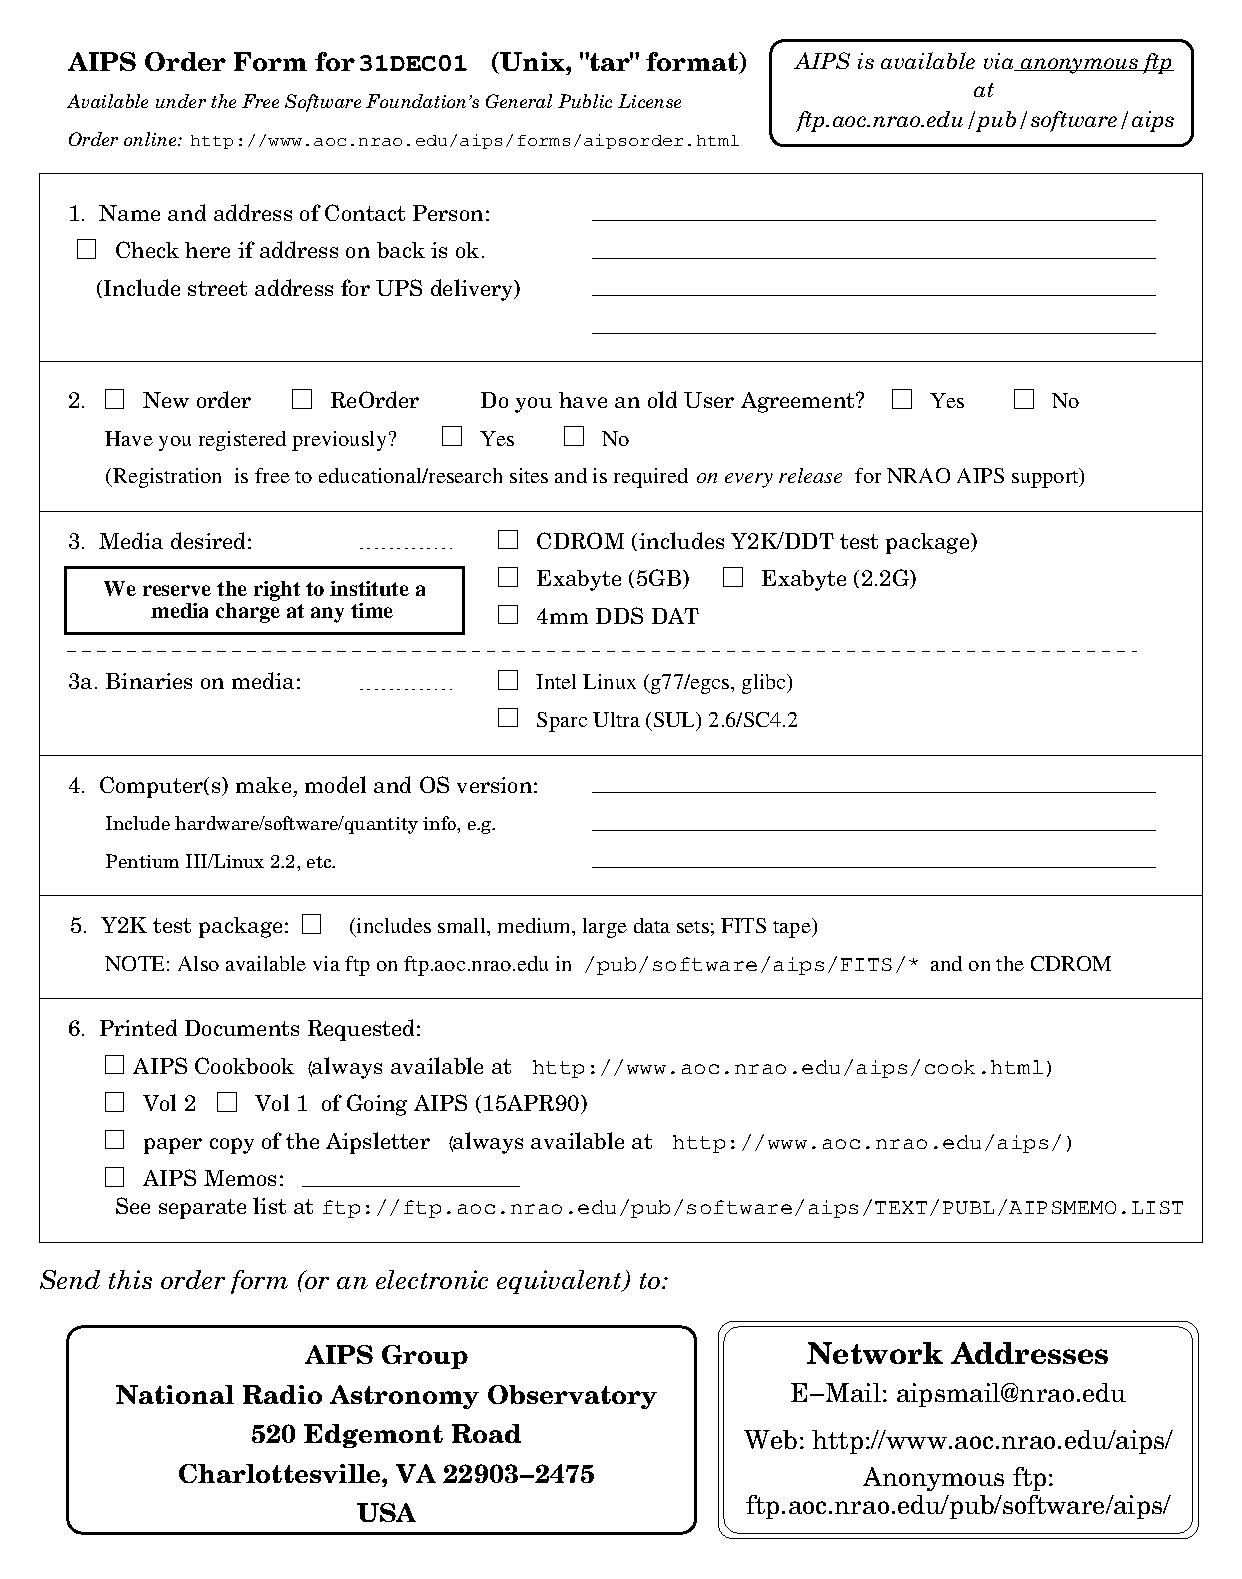
\includegraphics{FIG/AIPSORDER.PS}}}
\vfill\eject
\vbox to 4.4in{
\vspace{12pt}
%\centerline{\rotatebox{-90}{\resizebox{!}{3.5in}{%
%\includegraphics{FIG/Mandrill.color.plt}}}}
\centerline{\resizebox{!}{3.5in}{\includegraphics{FIG/Mandrill.eps}}}
\vspace{12pt}
\centerline{{\huge \tt \AIPRELEASE}}
\vspace{12pt}
\vfill}
\phantom{...}
\centerline{\resizebox{!}{!}{\includegraphics{FIG/AIPSLETS.PS}}}

\end{document}

